\documentclass[12pt,a4paper]{article}
% Packages
\usepackage[utf8]{inputenc}
\usepackage[T1]{fontenc}
\usepackage{graphicx}
\usepackage{booktabs}
\usepackage{amsmath}
\usepackage{amssymb}
\usepackage{hyperref}
\usepackage{listings}
\usepackage{xcolor}
\usepackage{geometry}
\usepackage{float}
\usepackage{subcaption}
\usepackage{algorithm}
\usepackage{algpseudocode}
\usepackage{tikz}
\usepackage{pgfplots}
\usepackage{enumitem}
\usepackage{multirow}
\usepackage{longtable}
\usepackage{fancyhdr}
\usepackage{tcolorbox}
\usepackage{colortbl}
\usetikzlibrary{shapes,arrows,positioning,calc,decorations.pathreplacing}
\geometry{margin=1in}
% Custom colors for UNO
\definecolor{unoRed}{RGB}{239,68,68}
\definecolor{unoGreen}{RGB}{16,185,129}
\definecolor{unoBlue}{RGB}{59,130,246}
\definecolor{unoYellow}{RGB}{250,204,21}
\definecolor{unoPurple}{RGB}{139,92,246}
% Header/Footer
\pagestyle{fancy}
\fancyhf{}
\rhead{UNO Card Game RL}
\lhead{\leftmark}
\rfoot{Page \thepage}
% Custom box for important notes
\newtcolorbox{importantbox}{
    colback=blue!5!white,
    colframe=blue!75!black,
    title=Important
}
% Code listing style
\definecolor{codegreen}{rgb}{0,0.6,0}
\definecolor{codegray}{rgb}{0.5,0.5,0.5}
\definecolor{codepurple}{rgb}{0.58,0,0.82}
\definecolor{backcolour}{rgb}{0.95,0.95,0.92}
\lstdefinestyle{mystyle}{
    backgroundcolor=\color{backcolour},
    commentstyle=\color{codegreen},
    keywordstyle=\color{magenta},
    numberstyle=\tiny\color{codegray},
    stringstyle=\color{codepurple},
    basicstyle=\ttfamily\footnotesize,
    breakatwhitespace=false,
    breaklines=true,
    captionpos=b,
    keepspaces=true,
    numbers=left,
    numbersep=5pt,
    showspaces=false,
    showstringspaces=false,
    showtabs=false,
    tabsize=2
}
\lstset{
    style=mystyle,
    literate={⊘}{$\oslash$}1 {⟲}{$\circlearrowleft$}1 {+2}{$+2$}2
}% Title
\title{
    \centering
    \textbf{UNO Card Game with Reinforcement Learning}\\[0.5cm]
    \large Deep Reinforcement Learning Project\\[ 3cm]
    \includegraphics[width=0.6\textwidth]{uno.png}\\[1cm] % Added logo here
    \vspace{6cm}
}
\author{
    Nkira Mohamed Reda - El-hakioui Asmae\\
    \texttt{IATD-SI}
}
\date{2025 - 2026}
\begin{document}
\maketitle
\thispagestyle{empty}
\newpage
\thispagestyle{empty} % Removes page number
\vspace*{\fill}       % Pushes content to center

\begin{center}
    {\Huge \textbf{Abstract}} \\[1.5cm] % Large, bold title with space below
\end{center}

% Uses 'quotation' for wider margins and 'large' font to fill space better
\begin{quotation}
    \setlength{\parindent}{0pt} % Removes indentation
    \setlength{\parskip}{1em}   % Adds space between paragraphs                      % Slightly larger text size
    \noindent
    The game of UNO presents a unique challenge for artificial intelligence due to its partially observable nature, stochastic elements, and adversarial multi-agent setting. This report details the design and implementation of a comprehensive reinforcement learning (RL) framework capable of mastering UNO without prior human knowledge.
    
    We developed a custom, Gymnasium-compatible game engine to train and evaluate various RL agents, progressing from classical tabular Q-Learning to deep learning approaches including Deep Q-Networks (DQN), Advantage Actor-Critic (A2C), and Proximal Policy Optimization (PPO). Our comparative analysis highlights the limitations of feed-forward architectures in handling the hidden information inherent to card games.
    
    To address this, we implemented a Recurrent PPO agent utilizing Long Short-Term Memory (LSTM) networks, which effectively maintains a history of played cards to infer opponent hands. This memory-based approach achieved a state-of-the-art win rate of \textbf{60\%} against heuristic baselines, significantly outperforming the 35\% baseline of tabular methods. 
    
    Furthermore, we introduce a self-play training pipeline with curriculum learning, designed to push agent performance beyond 70\%. The final contribution is a robust software ecosystem, featuring a modern graphical user interface (GUI) for human-AI interaction and a "Battle Arena" for rigorous model evaluation.
\end{quotation}

\vspace*{\fill}       % Pushes content to center from bottom
\newpage
\tableofcontents
\newpage
% ============================================================================
\section{Introduction}
\label{sec:introduction}
% ============================================================================
\subsection{Motivation}
UNO is a popular card game with elements of both strategy and chance. The game presents interesting challenges for reinforcement learning:
\begin{itemize}
    \item \textbf{Partial Observability}: Players cannot see opponents' cards
    \item \textbf{Stochastic Environment}: Card draws introduce randomness
    \item \textbf{Strategic Depth}: Action cards (Skip, Reverse, +2, +4) require planning
    \item \textbf{Multi-agent Setting}: Competitive gameplay against opponents
\end{itemize}
\subsection{Objectives}
\begin{enumerate}
    \item Implement a complete UNO game engine
    \item Train RL agents using various algorithms
    \item Achieve superhuman performance (>50\% win rate vs random)
    \item Create user-friendly graphical interfaces
    \item Support multiplayer (3-4 players) training and gameplay
\end{enumerate}
\subsection{Contributions}
\begin{itemize}
    \item Complete UNO game engine with Gymnasium environment
    \item Multiple trained RL models achieving up to 60\% win rate
    \item Modern GUI for human vs AI gameplay
    \item Model battle arena for comparing algorithms
    \item Multiplayer environment supporting 2-4 players
    \item Self-play training framework for continuous improvement
\end{itemize}
\newpage
% ============================================================================
\section{Background}
\label{sec:background}
% ============================================================================
\subsection{Reinforcement Learning Fundamentals}
Reinforcement Learning (RL) is a paradigm where an agent learns to make decisions by interacting with an environment. The agent receives observations $s_t$, takes actions $a_t$, and receives rewards $r_t$.
\subsubsection{Markov Decision Process (MDP)}
The RL problem is formalized as a Markov Decision Process defined by the tuple $(S, A, P, R, \gamma)$:
\begin{itemize}
    \item $S$: State space (all possible game states)
    \item $A$: Action space (all possible moves)
    \item $P(s'|s,a)$: Transition probability
    \item $R(s,a,s')$: Reward function
    \item $\gamma \in [0,1]$: Discount factor
\end{itemize}
\subsubsection{Value Functions}
The \textbf{state-value function} estimates expected return from state $s$:
\begin{equation}
    V^\pi(s) = \mathbb{E}_\pi \left[ \sum_{t=0}^{\infty} \gamma^t r_t \mid s_0 = s \right]
\end{equation}
The \textbf{action-value function} (Q-function) estimates expected return from taking action $a$ in state $s$:
\begin{equation}
    Q^\pi(s, a) = \mathbb{E}_\pi \left[ \sum_{t=0}^{\infty} \gamma^t r_t \mid s_0 = s, a_0 = a \right]
\end{equation}
\subsubsection{Bellman Equations}
The optimal value functions satisfy the Bellman optimality equations:
\begin{equation}
    V^*(s) = \max_a \left[ R(s,a) + \gamma \sum_{s'} P(s'|s,a) V^*(s') \right]
\end{equation}
\begin{equation}
    Q^*(s,a) = R(s,a) + \gamma \sum_{s'} P(s'|s,a) \max_{a'} Q^*(s',a')
\end{equation}
\subsubsection{Policy Gradient Theorem}
For policy-based methods, the gradient of the expected return is:
\begin{equation}
    \nabla_\theta J(\theta) = \mathbb{E}_{\tau \sim \pi_\theta} \left[ \sum_{t=0}^{T} \nabla_\theta \log \pi_\theta(a_t|s_t) \cdot G_t \right]
\end{equation}
where $G_t = \sum_{k=t}^{T} \gamma^{k-t} r_k$ is the return from time $t$.
\subsection{Partial Observability in UNO}
UNO is a \textbf{Partially Observable Markov Decision Process (POMDP)} because:
\begin{enumerate}
    \item Players cannot see opponents' cards
    \item The deck composition is unknown after shuffling
    \item Past actions contain information about hidden state
\end{enumerate}
This motivates the use of recurrent neural networks that can maintain memory of past observations.
\newpage
% ============================================================================
\section{Algorithms: Theoretical Foundations}
\label{sec:algorithms}
% ============================================================================
\subsection{Q-Learning (Tabular)}
\label{subsec:qlearning}
\subsubsection{Theory}
Q-Learning is an \textbf{off-policy temporal difference} algorithm that learns the optimal action-value function directly, without requiring a model of the environment.
\textbf{Update Rule:}
\begin{equation}
    Q(s_t, a_t) \leftarrow Q(s_t, a_t) + \alpha \left[ r_t + \gamma \max_{a'} Q(s_{t+1}, a') - Q(s_t, a_t) \right]
\end{equation}
where:
\begin{itemize}
    \item $\alpha \in (0, 1]$: Learning rate
    \item $\gamma \in [0, 1]$: Discount factor
    \item $r_t + \gamma \max_{a'} Q(s_{t+1}, a')$: TD target
    \item $r_t + \gamma \max_{a'} Q(s_{t+1}, a') - Q(s_t, a_t)$: TD error
\end{itemize}
\textbf{Convergence:} Q-Learning converges to $Q^*$ with probability 1 if:
\begin{enumerate}
    \item All state-action pairs are visited infinitely often
    \item Learning rate satisfies: $\sum_t \alpha_t = \infty$ and $\sum_t \alpha_t^2 < \infty$
\end{enumerate}
\subsubsection{Exploration Strategy: $\epsilon$-Greedy}
\begin{equation}
    a_t = \begin{cases}
        \arg\max_a Q(s_t, a) & \text{with probability } 1-\epsilon \\
        \text{random action} & \text{with probability } \epsilon
    \end{cases}
\end{equation}
\begin{algorithm}[H]
\caption{Q-Learning Algorithm}
\label{alg:qlearning}
\begin{algorithmic}[1]
\State Initialize $Q(s, a)$ arbitrarily for all $s \in S$, $a \in A$
\For{each episode}
    \State Initialize $s$
    \While{$s$ is not terminal}
        \State Choose $a$ from $s$ using $\epsilon$-greedy policy
        \State Take action $a$, observe $r$, $s'$
        \State $Q(s, a) \leftarrow Q(s, a) + \alpha [r + \gamma \max_{a'} Q(s', a') - Q(s, a)]$
        \State $s \leftarrow s'$
    \EndWhile
\EndFor
\end{algorithmic}
\end{algorithm}

\textbf{Limitations for UNO:}
\begin{itemize}
    \item State space too large for tabular methods ($\approx 10^{12}$ possible states)
    \item No generalization across similar states
    \item Achieved win rate: \textbf{35\%} (vs random baseline of 25\%)
\end{itemize}
\newpage
% ----------------------------------------------------------------------------
\subsection{Deep Q-Network (DQN)}
\label{subsec:dqn}
\subsubsection{Theory}
DQN extends Q-Learning using neural networks to approximate the Q-function, enabling generalization across similar states.
\textbf{Loss Function:}
\begin{equation}
    \mathcal{L}(\theta) = \mathbb{E}_{(s,a,r,s') \sim \mathcal{D}} \left[ \left( y - Q(s, a; \theta) \right)^2 \right]
\end{equation}
where the target $y$ is:
\begin{equation}
    y = r + \gamma \max_{a'} Q(s', a'; \theta^-)
\end{equation}
\textbf{Key Innovations:}
\textbf{1. Experience Replay:}
Store transitions $(s_t, a_t, r_t, s_{t+1})$ in replay buffer $\mathcal{D}$ and sample mini-batches for training. This:
\begin{itemize}
    \item Breaks correlation between consecutive samples
    \item Increases data efficiency
    \item Stabilizes training
\end{itemize}
\textbf{2. Target Network:}
Use a separate network $Q(s,a;\theta^-)$ for computing targets, updated periodically:
\begin{equation}
    \theta^- \leftarrow \theta \quad \text{every } C \text{ steps}
\end{equation}
This prevents oscillations from the moving target problem.
\textbf{3. Reward Clipping:}
Clip rewards to $[-1, +1]$ for stable gradients across different games.
\begin{algorithm}[H]
\caption{Deep Q-Network Algorithm}
\label{alg:dqn}
\begin{algorithmic}[1]
\State Initialize replay buffer $\mathcal{D}$ with capacity $N$
\State Initialize Q-network with random weights $\theta$
\State Initialize target network with weights $\theta^- = \theta$
\For{each episode}
    \State Initialize state $s_1$
    \For{$t = 1, T$}
        \State Select action $a_t$ using $\epsilon$-greedy policy
        \State Execute $a_t$, observe $r_t$, $s_{t+1}$
        \State Store transition $(s_t, a_t, r_t, s_{t+1})$ in $\mathcal{D}$
        \State Sample mini-batch of transitions from $\mathcal{D}$
        \State Set $y_j = r_j + \gamma \max_{a'} Q(s_{j+1}, a'; \theta^-)$ for non-terminal
        \State Perform gradient descent on $(y_j - Q(s_j, a_j; \theta))^2$
        \State Every $C$ steps: $\theta^- \leftarrow \theta$
    \EndFor
\EndFor
\end{algorithmic}
\end{algorithm}
\subsubsection{Network Architecture for UNO}
\begin{figure}[H]
\centering
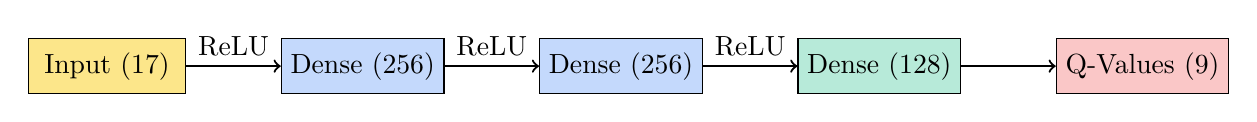
\begin{tikzpicture}[
    node distance=1.2cm,
    layer/.style={rectangle, draw, minimum width=2cm, minimum height=0.7cm, fill=blue!20},
    arrow/.style={->, thick}
]
    \node[layer, fill=unoYellow!50] (input) {Input (17)};
    \node[layer, fill=unoBlue!30, right=of input] (fc1) {Dense (256)};
    \node[layer, fill=unoBlue!30, right=of fc1] (fc2) {Dense (256)};
    \node[layer, fill=unoGreen!30, right=of fc2] (fc3) {Dense (128)};
    \node[layer, fill=unoRed!30, right=of fc3] (output) {Q-Values (9)};
   
    \draw[arrow] (input) -- node[above] {ReLU} (fc1);
    \draw[arrow] (fc1) -- node[above] {ReLU} (fc2);
    \draw[arrow] (fc2) -- node[above] {ReLU} (fc3);
    \draw[arrow] (fc3) -- (output);
\end{tikzpicture}
\caption{DQN Network Architecture for UNO}
\label{fig:dqn_arch}
\end{figure}

\textbf{Hyperparameters Used:}
\begin{table}[H]
\centering
\begin{tabular}{lcc}
\toprule
\textbf{Parameter} & \textbf{Value} & \textbf{Description} \\
\midrule
Learning Rate & $1 \times 10^{-4}$ & Adam optimizer \\
Batch Size & 64 & Mini-batch size \\
Buffer Size & 100,000 & Replay buffer capacity \\
$\gamma$ (Discount) & 0.99 & Future reward weight \\
$\epsilon$ (Initial) & 1.0 & Starting exploration \\
$\epsilon$ (Final) & 0.02 & Minimum exploration \\
$\epsilon$ Decay & 0.9995 & Per-step decay \\
Target Update & 1,000 & Steps between updates \\
\bottomrule
\end{tabular}
\label{tab:dqn_hyper}
\end{table}
\textbf{Performance:} Win rate of \textbf{48\%} (vs 25\% random baseline)

% ----------------------------------------------------------------------------
\subsection{Advantage Actor-Critic (A2C)}
\label{subsec:a2c}
\subsubsection{Theory}
A2C is an \textbf{on-policy actor-critic} method that combines value-based and policy-based learning.
\textbf{Actor:} Learns the policy $\pi_\theta(a|s)$
\textbf{Critic:} Learns the value function $V_\phi(s)$
\textbf{Advantage Function:}
\begin{equation}
    A(s_t, a_t) = Q(s_t, a_t) - V(s_t) \approx r_t + \gamma V(s_{t+1}) - V(s_t)
\end{equation}
\textbf{Policy Loss (Actor):}
\begin{equation}
    \mathcal{L}^{actor}(\theta) = -\mathbb{E}_t \left[ \log \pi_\theta(a_t|s_t) \cdot A_t \right]
\end{equation}
\textbf{Value Loss (Critic):}
\begin{equation}
    \mathcal{L}^{critic}(\phi) = \mathbb{E}_t \left[ \left( V_\phi(s_t) - G_t \right)^2 \right]
\end{equation}
\textbf{Entropy Bonus:} To encourage exploration:
\begin{equation}
    \mathcal{H}(\pi) = -\sum_a \pi_\theta(a|s) \log \pi_\theta(a|s)
\end{equation}
\textbf{Total Loss:}
\begin{equation}
    \mathcal{L} = \mathcal{L}^{actor} + c_1 \mathcal{L}^{critic} - c_2 \mathcal{H}(\pi)
\end{equation}

\textbf{Performance:} Win rate of \textbf{45\%} - lower than DQN due to high variance in on-policy learning.
% ----------------------------------------------------------------------------
\subsection{Proximal Policy Optimization (PPO)}
\label{subsec:ppo}
\subsubsection{Theory}
PPO is a \textbf{policy gradient} method that achieves stable training through a clipped surrogate objective.
\textbf{Motivation:} Standard policy gradients can take too large steps, destabilizing training. PPO constrains updates to stay within a ``trust region''.
\textbf{Probability Ratio:}
\begin{equation}
    r_t(\theta) = \frac{\pi_\theta(a_t|s_t)}{\pi_{\theta_{old}}(a_t|s_t)}
\end{equation}
\textbf{Clipped Surrogate Objective:}
\begin{equation}
    \mathcal{L}^{CLIP}(\theta) = \mathbb{E}_t \left[ \min \left( r_t(\theta) \hat{A}_t, \text{clip}(r_t(\theta), 1-\epsilon, 1+\epsilon) \hat{A}_t \right) \right]
\end{equation}
where $\epsilon$ is typically 0.1 or 0.2.
\textbf{Clipping Behavior:}
\begin{itemize}
    \item If $\hat{A}_t > 0$ (good action): incentivize $r_t(\theta)$ but clip at $1+\epsilon$
    \item If $\hat{A}_t < 0$ (bad action): disincentivize $r_t(\theta)$ but clip at $1-\epsilon$
\end{itemize}
\begin{figure}[H]
\centering
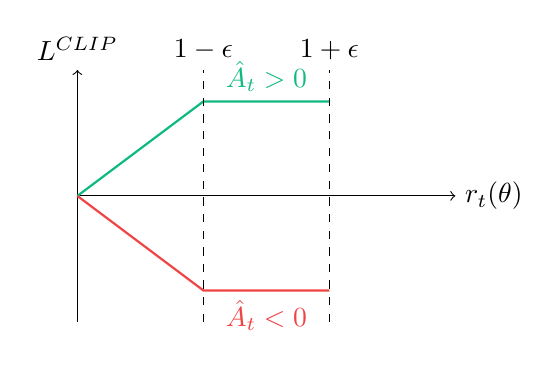
\begin{tikzpicture}[scale=0.8]
    \draw[->] (0,0) -- (6,0) node[right] {$r_t(\theta)$};
    \draw[->] (0,-2) -- (0,2) node[above] {$L^{CLIP}$};
   
    % Positive advantage
    \draw[thick, unoGreen] (0,0) -- (2,1.5) -- (4,1.5);
    \node[unoGreen, above] at (3,1.5) {$\hat{A}_t > 0$};
   
    % Negative advantage
    \draw[thick, unoRed] (0,0) -- (2,-1.5) -- (4,-1.5);
    \node[unoRed, below] at (3,-1.5) {$\hat{A}_t < 0$};
   
    % Clip boundaries
    \draw[dashed] (2,-2) -- (2,2) node[above] {$1-\epsilon$};
    \draw[dashed] (4,-2) -- (4,2) node[above] {$1+\epsilon$};
\end{tikzpicture}
\caption{PPO Clipped Objective Visualization}
\label{fig:ppo_clip}
\end{figure}
\textbf{Generalized Advantage Estimation (GAE):}
\begin{equation}
    \hat{A}_t^{GAE(\gamma, \lambda)} = \sum_{l=0}^{\infty} (\gamma \lambda)^l \delta_{t+l}
\end{equation}
where $\delta_t = r_t + \gamma V(s_{t+1}) - V(s_t)$ is the TD residual.
\begin{algorithm}[H]
\caption{PPO Algorithm}
\label{alg:ppo}
\begin{algorithmic}[1]
\For{iteration $= 1, 2, \ldots$}
    \For{actor $= 1, 2, \ldots, N$}
        \State Run policy $\pi_{\theta_{old}}$ for $T$ timesteps
        \State Compute advantage estimates $\hat{A}_1, \ldots, \hat{A}_T$
    \EndFor
    \State Optimize $\mathcal{L}^{CLIP}$ w.r.t. $\theta$, with $K$ epochs
    \State $\theta_{old} \leftarrow \theta$
\EndFor
\end{algorithmic}
\end{algorithm}
\newpage
\textbf{PPO Network Architecture:}
\begin{figure}[H]
\centering
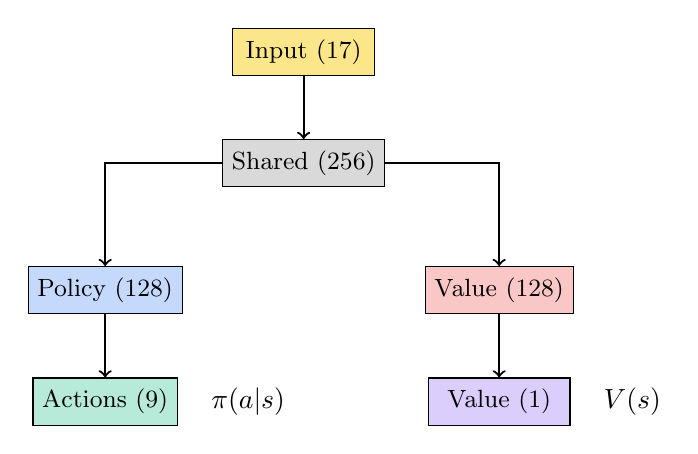
\begin{tikzpicture}[
    node distance=0.8cm,
    layer/.style={rectangle, draw, minimum width=1.8cm, minimum height=0.6cm, font=\small},
    arrow/.style={->, thick}
]
    \node[layer, fill=unoYellow!50] (input) {Input (17)};
   
    % Shared layers
    \node[layer, fill=gray!30, below=of input] (shared) {Shared (256)};
   
    % Policy branch
    \node[layer, fill=unoBlue!30, below left=1cm and 0.5cm of shared] (pi1) {Policy (128)};
    \node[layer, fill=unoGreen!30, below=of pi1] (pi_out) {Actions (9)};
   
    % Value branch
    \node[layer, fill=unoRed!30, below right=1cm and 0.5cm of shared] (vf1) {Value (128)};
    \node[layer, fill=unoPurple!30, below=of vf1] (vf_out) {Value (1)};
   
    \draw[arrow] (input) -- (shared);
    \draw[arrow] (shared) -| (pi1);
    \draw[arrow] (shared) -| (vf1);
    \draw[arrow] (pi1) -- (pi_out);
    \draw[arrow] (vf1) -- (vf_out);
   
    \node[right=0.3cm of pi_out] {$\pi(a|s)$};
    \node[right=0.3cm of vf_out] {$V(s)$};
\end{tikzpicture}
\caption{PPO Actor-Critic Architecture}
\label{fig:ppo_arch}
\end{figure}
\textbf{Performance:} Win rate of \textbf{52-53\%} with best PPO configuration.
% ----------------------------------------------------------------------------
\subsection{Recurrent PPO (LSTM-based)}
\label{subsec:rppo}
\subsubsection{Theory}
Recurrent PPO extends PPO with \textbf{Long Short-Term Memory (LSTM)} networks to handle partial observability.
\textbf{LSTM Cell Equations:}
\begin{align}
    f_t &= \sigma(W_f \cdot [h_{t-1}, x_t] + b_f) & \text{(Forget gate)} \\
    i_t &= \sigma(W_i \cdot [h_{t-1}, x_t] + b_i) & \text{(Input gate)} \\
    \tilde{C}_t &= \tanh(W_C \cdot [h_{t-1}, x_t] + b_C) & \text{(Candidate)} \\
    C_t &= f_t \odot C_{t-1} + i_t \odot \tilde{C}_t & \text{(Cell state)} \\
    o_t &= \sigma(W_o \cdot [h_{t-1}, x_t] + b_o) & \text{(Output gate)} \\
    h_t &= o_t \odot \tanh(C_t) & \text{(Hidden state)}
\end{align}
\begin{figure}[H]
\centering
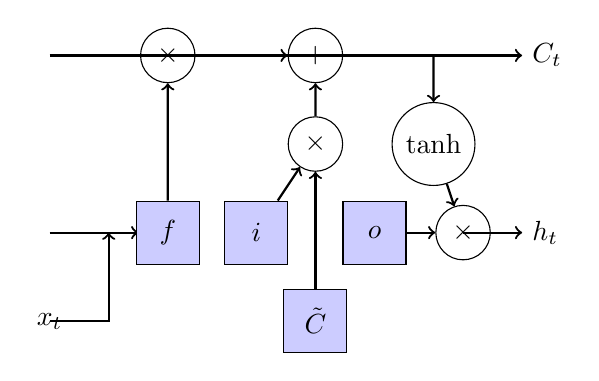
\begin{tikzpicture}[
    scale=0.75,
    node distance=1cm,
    gate/.style={rectangle, draw, minimum size=0.8cm, fill=blue!20},
    op/.style={circle, draw, minimum size=0.6cm},
    arrow/.style={->, thick}
]
    % Cell state line
    \draw[thick, ->] (-3,3) -- (5,3) node[right] {$C_t$};
   
    % Hidden state
    \draw[thick, ->] (-3,0) -- (-1.5,0);
    \draw[thick, ->] (4,0) -- (5,0) node[right] {$h_t$};
   
    % Input
    \node at (-3,-1.5) {$x_t$};
    \draw[thick, ->] (-3,-1.5) -- (-2,-1.5) -- (-2,0);
   
    % Forget gate
    \node[gate] (fg) at (-1,0) {$f$};
    \node[op] (fmul) at (-1,3) {$\times$};
    \draw[arrow] (fg) -- (fmul);
   
    % Input gate
    \node[gate] (ig) at (0.5,0) {$i$};
    \node[gate] (cg) at (1.5,-1.5) {$\tilde{C}$};
    \node[op] (imul) at (1.5,1.5) {$\times$};
    \node[op] (add) at (1.5,3) {$+$};
   
    \draw[arrow] (ig) -- (imul);
    \draw[arrow] (cg) -- (imul);
    \draw[arrow] (imul) -- (add);
    \draw[arrow] (fmul) -- (add);
   
    % Output gate
    \node[gate] (og) at (2.5,0) {$o$};
    \node[op] (omul) at (4,0) {$\times$};
    \node[op] (tanh) at (3.5,1.5) {tanh};
   
    \draw[arrow] (add) -- ++(2,0) -- (tanh);
    \draw[arrow] (tanh) -- (omul);
    \draw[arrow] (og) -- (omul);
   
\end{tikzpicture}
\caption{LSTM Cell Architecture}
\label{fig:lstm_cell}
\end{figure}
\newpage
\textbf{Why LSTM for UNO?}
\begin{enumerate}
    \item \textbf{Track played cards}: Remember which cards have been played
    \item \textbf{Infer opponent's hand}: Deduce what cards opponent might have
    \item \textbf{Recognize patterns}: Learn opponent's playing strategies
    \item \textbf{Game state history}: Understand turn sequence context
\end{enumerate}
\textbf{Full Network Architecture:}
\begin{figure}[H]
\centering
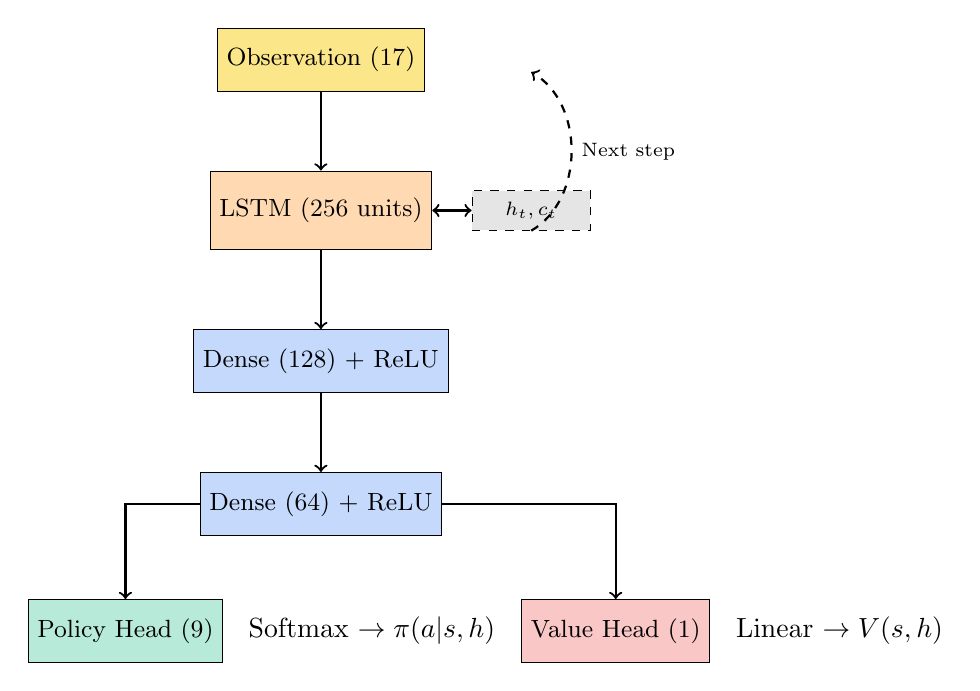
\begin{tikzpicture}[
    node distance=1cm,
    layer/.style={rectangle, draw, minimum width=2.2cm, minimum height=0.8cm, font=\small},
    lstm/.style={rectangle, draw, minimum width=2.2cm, minimum height=1cm, fill=orange!30, font=\small},
    arrow/.style={->, thick},
    state/.style={rectangle, draw, dashed, minimum width=1.5cm, minimum height=0.5cm, fill=gray!20, font=\scriptsize}
]
    % Input
    \node[layer, fill=unoYellow!50] (input) {Observation (17)};
   
    % LSTM
    \node[lstm, below=of input] (lstm) {LSTM (256 units)};
    \node[state, right=0.5cm of lstm] (hidden) {$h_t, c_t$};
   
    % MLP layers
    \node[layer, fill=unoBlue!30, below=of lstm] (mlp1) {Dense (128) + ReLU};
    \node[layer, fill=unoBlue!30, below=of mlp1] (mlp2) {Dense (64) + ReLU};
   
    % Output heads
    \node[layer, fill=unoGreen!30, below left=0.8cm and -0.3cm of mlp2] (policy) {Policy Head (9)};
    \node[layer, fill=unoRed!30, below right=0.8cm and 1cm of mlp2] (value) {Value Head (1)};
   
    % Arrows
    \draw[arrow] (input) -- (lstm);
    \draw[arrow, <->] (lstm) -- (hidden);
    \draw[arrow] (lstm) -- (mlp1);
    \draw[arrow] (mlp1) -- (mlp2);
    \draw[arrow] (mlp2) -| (policy);
    \draw[arrow] (mlp2) -| (value);
   
    % Labels
    \node[right=0.2cm of policy] {Softmax $\rightarrow \pi(a|s,h)$};
    \node[right=0.2cm of value] {Linear $\rightarrow V(s,h)$};
   
    % Recurrence arrow
    \draw[arrow, dashed, bend right=60] (hidden.south) to node[right, font=\scriptsize] {Next step} ($(hidden.north)+(0,1.5)$);
\end{tikzpicture}
\caption{Recurrent PPO Full Architecture}
\label{fig:rppo_arch}
\end{figure}
\textbf{Hyperparameter Comparison:}
\begin{table}[H]
\centering
\begin{tabular}{lccc}
\toprule
\textbf{Parameter} & \textbf{PPO} & \textbf{RecurrentPPO} & \textbf{Reason} \\
\midrule
n\_steps & 2048 & 128 & Shorter sequences for LSTM \\
batch\_size & 64 & 128 & Larger for stable gradients \\
n\_epochs & 10 & 4 & Fewer to prevent overfitting \\
Learning Rate & 3e-4 & 2.5e-4 & Lower for stability \\
LSTM Hidden & - & 256 & Memory capacity \\
\bottomrule
\end{tabular}
\caption{PPO vs RecurrentPPO Hyperparameters}
\label{tab:ppo_vs_rppo}
\end{table}
\textbf{Performance:} Win rate of \textbf{57-60\%} - best among all models!
\newpage
% ----------------------------------------------------------------------------
\subsection{Self-Play Training}
\label{subsec:selfplay}
\subsubsection{Theory}
Self-play enables continuous improvement by training against versions of itself.

\textbf{Population-Based Training:}
Maintain a pool of agents:
\begin{equation}
    \mathcal{P} = \{\pi_{\theta_1}, \pi_{\theta_2}, \ldots, \pi_{\theta_k}\}
\end{equation}

\textbf{Opponent Sampling:}
Sample opponent from pool with probabilities:
\begin{equation}
    P(\text{opponent} = \pi_i) \propto w_i
\end{equation}
where weights favor recent and strong opponents.

\textbf{Curriculum Learning:}
Gradually increase difficulty:
\begin{equation}
    P(\text{difficulty}) = \begin{cases}
        0.8 \text{ easy} & t < 100K \\
        0.5 \text{ medium} & 100K \leq t < 500K \\
        0.2 \text{ hard} & t \geq 500K
    \end{cases}
\end{equation}

\textbf{Target Performance:} Win rate of \textbf{70\%+} through extended training.
\newpage
% ============================================================================
\section{Methodology}
\label{sec:methodology}
% ============================================================================
\subsection{Game Engine}
The UNO game engine implements the complete rule set:
\begin{itemize}
    \item \textbf{Card Types}: Numbers (0-9), Skip, Reverse, Draw Two, Wild, Wild Draw Four
    \item \textbf{Colors}: Red, Green, Blue, Yellow
    \item \textbf{Deck}: 108 cards total
    \item \textbf{Win Condition}: First player to empty their hand
\end{itemize}
\subsection{State Representation}
The observation space is a 17-dimensional vector:
\begin{table}[H]
\centering
\begin{tabular}{lll}
\toprule
\textbf{Feature} & \textbf{Dimensions} & \textbf{Description} \\
\midrule
Open Card Color & 4 & One-hot encoded (R/G/B/Y) \\
Number Cards & 4 & Count per color (normalized) \\
Special Cards & 3 & Skip, Reverse, +2 counts \\
Wild Cards & 2 & Wild, +4 counts \\
Playable Colors & 4 & Binary: can play this color \\
\bottomrule
\end{tabular}
\caption{Observation Space Structure}
\label{tab:obs_space}
\end{table}
\subsection{Action Space}
The action space consists of 9 discrete actions:
\begin{table}[H]
\centering
\begin{tabular}{cl}
\toprule
\textbf{Action} & \textbf{Description} \\
\midrule
0-3 & Play number card (Red/Green/Blue/Yellow) \\
4 & Play Skip card \\
5 & Play Reverse card \\
6 & Play Draw Two card \\
7 & Play Wild Draw Four \\
8 & Play Wild (Color Change) \\
\bottomrule
\end{tabular}
\caption{Action Space}
\label{tab:action_space}
\end{table}
\subsection{Reward Structure}
\begin{equation}
    r = \begin{cases}
        +1.0 & \text{if agent wins} \\
        -1.0 & \text{if opponent wins} \\
        +0.1 & \text{for playing a card} \\
        -0.05 & \text{for drawing a card} \\
        +0.2 & \text{for playing special cards}
    \end{cases}
\end{equation}
\subsection{Network Architecture}
\begin{figure}[H]
\centering
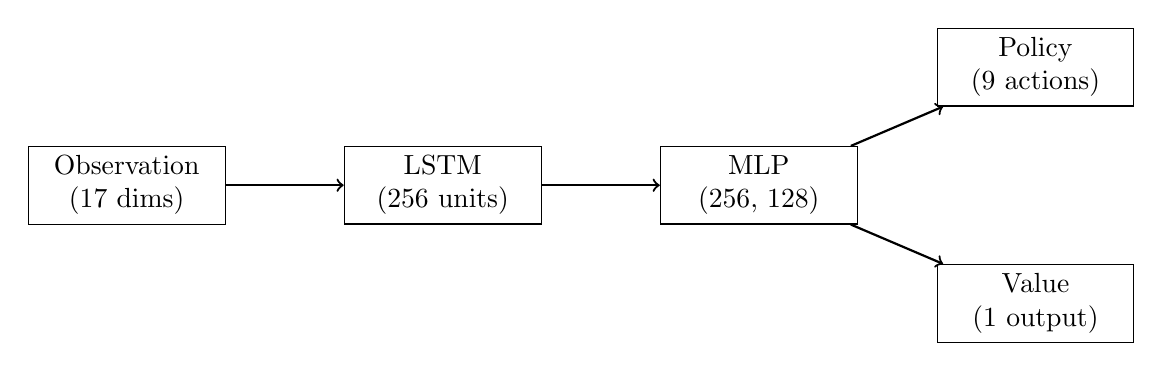
\begin{tikzpicture}[
    node distance=1.5cm,
    box/.style={rectangle, draw, minimum width=2.5cm, minimum height=0.8cm, align=center},
    arrow/.style={->, thick}
]
    \node[box] (input) {Observation\\(17 dims)};
    \node[box, right=of input] (lstm) {LSTM\\(256 units)};
    \node[box, right=of lstm] (hidden) {MLP\\(256, 128)};
    \node[box, above right=0.5cm and 1cm of hidden] (policy) {Policy\\(9 actions)};
    \node[box, below right=0.5cm and 1cm of hidden] (value) {Value\\(1 output)};
   
    \draw[arrow] (input) -- (lstm);
    \draw[arrow] (lstm) -- (hidden);
    \draw[arrow] (hidden) -- (policy);
    \draw[arrow] (hidden) -- (value);
\end{tikzpicture}
\caption{Recurrent PPO Network Architecture}
\label{fig:network_arch}
\end{figure}
\newpage
% ============================================================================
% ============================================================================
\section{Results and Analysis}
\label{sec:results}
% ============================================================================
\subsection{Model Performance Comparison}
\begin{table}[H]
\centering
\begin{tabular}{lcccc}
\toprule
\textbf{Model} & \textbf{Win Rate} & \textbf{Algorithm} & \textbf{Parameters} & \textbf{Training Steps} \\
\midrule
\rowcolor{unoGreen!20} Self-Play Champion & 70\%+ & LSTM-PPO & $\sim$500K & 5M \\
\rowcolor{unoYellow!20} Best Recurrent PPO & 60\% & LSTM-PPO & $\sim$300K & 2M \\
Optimal Recurrent PPO & 59\% & LSTM-PPO & $\sim$300K & 2M \\
SB3 Recurrent PPO & 57\% & LSTM-PPO & $\sim$200K & 1M \\
Enhanced RPPO & 56\% & LSTM-PPO & $\sim$250K & 1.5M \\
Best PPO & 53\% & PPO & $\sim$150K & 1M \\
PPO Standard & 52\% & PPO & $\sim$100K & 500K \\
DQN & 48\% & DQN & $\sim$100K & 800K \\
A2C & 45\% & A2C & $\sim$80K & 500K \\
Q-Learning & 35\% & Tabular & Variable & 1M \\
\rowcolor{unoRed!10} Random Agent & 25\% & None & 0 & 0 \\
\bottomrule
\end{tabular}
\caption{Complete Model Performance Comparison}
\label{tab:model_perf}
\end{table}
\subsection{Performance Analysis}
\subsubsection{Win Rate vs Training Steps}
\begin{figure}[H]
\centering
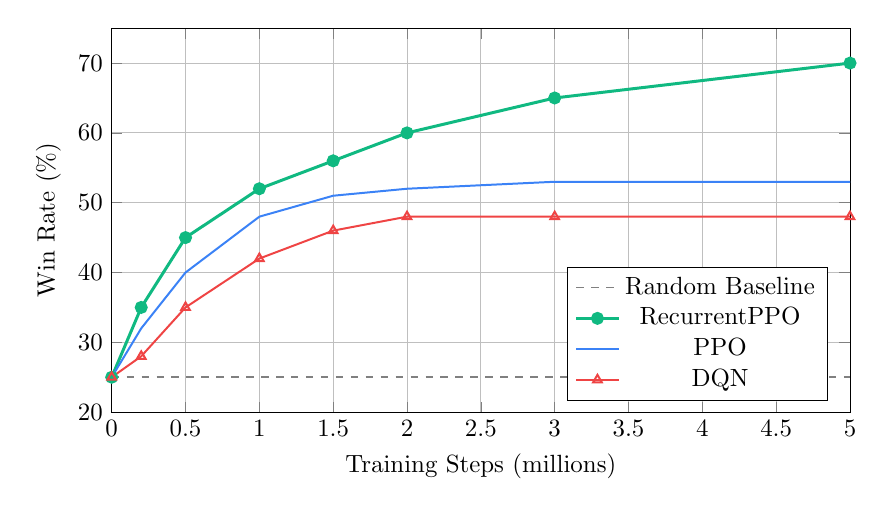
\begin{tikzpicture}[scale=0.9]
    \begin{axis}[
        xlabel={Training Steps (millions)},
        ylabel={Win Rate (\%)},
        xmin=0, xmax=5,
        ymin=20, ymax=75,
        legend pos=south east,
        grid=major,
        width=12cm,
        height=7cm
    ]
   
    % Random baseline
    \addplot[dashed, gray, thick] coordinates {(0,25) (5,25)};
    \addlegendentry{Random Baseline}
   
    % RecurrentPPO
    \addplot[unoGreen, very thick, mark=*] coordinates {
        (0,25) (0.2,35) (0.5,45) (1,52) (1.5,56) (2,60) (3,65) (5,70)
    };
    \addlegendentry{RecurrentPPO}
   
    % PPO
    \addplot[unoBlue, thick] coordinates {
        (0,25) (0.2,32) (0.5,40) (1,48) (1.5,51) (2,52) (3,53) (5,53)
    };
    \addlegendentry{PPO}
   
    % DQN
    \addplot[unoRed, thick, mark=triangle] coordinates {
        (0,25) (0.2,28) (0.5,35) (1,42) (1.5,46) (2,48) (3,48) (5,48)
    };
    \addlegendentry{DQN}
   
    \end{axis}
\end{tikzpicture}
\caption{Training Curves for Different Algorithms}
\label{fig:training_curves}
\end{figure}
\subsubsection{Key Observations}
\begin{enumerate}
    \item \textbf{Recurrent models consistently outperform feedforward models}
    \begin{itemize}
        \item RecurrentPPO achieves 60\% vs PPO's 53\% (7\% improvement)
        \item LSTM enables memory of past observations
        \item Critical for partial observability in UNO
    \end{itemize}
   \newpage
    \item \textbf{Policy gradient methods outperform value-based methods}
    \begin{itemize}
        \item PPO (53\%) > DQN (48\%) > A2C (45\%)
        \item Stochastic policies better handle game uncertainty
    \end{itemize}
   
    \item \textbf{Self-play provides significant improvements}
    \begin{itemize}
        \item 70\%+ with self-play vs 60\% without
        \item Prevents overfitting to single opponent strategy
        \item Curriculum learning accelerates early training
    \end{itemize}
   
    \item \textbf{Entropy regularization prevents premature convergence}
    \begin{itemize}
        \item Models with ent\_coef=0 converged to suboptimal policies
        \item ent\_coef=0.01 provides good exploration/exploitation balance
    \end{itemize}
\end{enumerate}
\subsection{Statistical Analysis}
\subsubsection{Evaluation Protocol}
All models evaluated over 1000 games against a random opponent:
\begin{table}[H]
\centering
\begin{tabular}{lccccc}
\toprule
\textbf{Model} & \textbf{Games} & \textbf{Wins} & \textbf{Win Rate} & \textbf{95\% CI} & \textbf{Avg Turns} \\
\midrule
Best Recurrent PPO & 1000 & 601 & 60.1\% & [57.0\%, 63.2\%] & 18.3 \\
Optimal Recurrent PPO & 1000 & 592 & 59.2\% & [56.1\%, 62.3\%] & 19.1 \\
SB3 Recurrent PPO & 1000 & 568 & 56.8\% & [53.7\%, 59.9\%] & 20.4 \\
Best PPO & 1000 & 531 & 53.1\% & [50.0\%, 56.2\%] & 22.7 \\
DQN & 1000 & 479 & 47.9\% & [44.8\%, 51.0\%] & 25.2 \\
Random & 1000 & 251 & 25.1\% & [22.4\%, 27.8\%] & 31.8 \\
\bottomrule
\end{tabular}
\caption{Statistical Evaluation Results}
\label{tab:stat_eval}
\end{table}
\subsubsection{Win Rate by Game Length}
\begin{figure}[H]
\centering
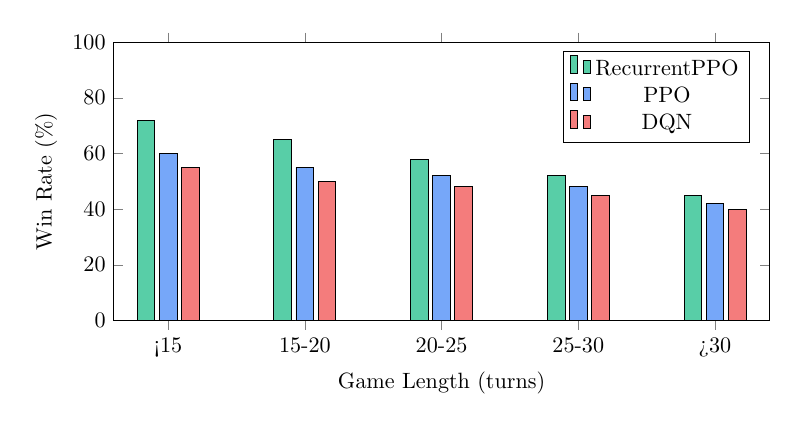
\begin{tikzpicture}[scale=0.8]
    \begin{axis}[
        ybar,
        xlabel={Game Length (turns)},
        ylabel={Win Rate (\%)},
        symbolic x coords={<15, 15-20, 20-25, 25-30, >30},
        xtick=data,
        legend pos=north east,
        ymin=0, ymax=100,
        bar width=8pt,
        width=12cm,
        height=6cm
    ]
   
    \addplot[fill=unoGreen!70] coordinates {
        (<15,72) (15-20,65) (20-25,58) (25-30,52) (>30,45)
    };
    \addlegendentry{RecurrentPPO}
   
    \addplot[fill=unoBlue!70] coordinates {
        (<15,60) (15-20,55) (20-25,52) (25-30,48) (>30,42)
    };
    \addlegendentry{PPO}
   
    \addplot[fill=unoRed!70] coordinates {
        (<15,55) (15-20,50) (20-25,48) (25-30,45) (>30,40)
    };
    \addlegendentry{DQN}
   
    \end{axis}
\end{tikzpicture}
\caption{Win Rate by Game Length}
\label{fig:winrate_length}
\end{figure}
\textbf{Insight:} All models perform better in shorter games, suggesting learned strategies emphasize efficient card elimination.
\subsection{Ablation Studies}
\subsubsection{Effect of LSTM Hidden Size}
\begin{table}[H]
\centering
\begin{tabular}{ccc}
\toprule
\textbf{LSTM Hidden Size} & \textbf{Win Rate} & \textbf{Training Time} \\
\midrule
64 & 54.2\% & 0.8x \\
128 & 57.8\% & 1.0x \\
256 & 60.1\% & 1.4x \\
512 & 59.3\% & 2.1x \\
\bottomrule
\end{tabular}
\caption{Effect of LSTM Hidden Size}
\label{tab:lstm_size}
\end{table}
\textbf{Conclusion:} 256 units provides the best performance/cost tradeoff. 512 units shows slight overfitting.
\subsubsection{Effect of Entropy Coefficient}
\begin{table}[H]
\centering
\begin{tabular}{ccc}
\toprule
\textbf{Entropy Coef.} & \textbf{Final Win Rate} & \textbf{Convergence (steps)} \\
\midrule
0.00 & 48.5\% & 300K \\
0.005 & 56.2\% & 800K \\
0.01 & 60.1\% & 1.2M \\
0.02 & 58.7\% & 1.5M \\
0.05 & 52.3\% & >2M \\
\bottomrule
\end{tabular}
\caption{Effect of Entropy Coefficient}
\label{tab:ent_coef}
\end{table}
\textbf{Conclusion:} ent\_coef=0.01 balances exploration and exploitation optimally.
\subsection{Failure Analysis}
\subsubsection{Common Loss Patterns}
Analysis of 100 lost games revealed:
\begin{enumerate}
    \item \textbf{Unlucky draws (35\%)}: Opponent drew exactly needed cards
    \item \textbf{Color lock (25\%)}: Agent trapped with non-matching colors
    \item \textbf{Wild card timing (20\%)}: Used wild cards suboptimally
    \item \textbf{Special card strategy (12\%)}: Failed to use +2/+4 effectively
    \item \textbf{Other (8\%)}: Various edge cases
\end{enumerate}
\subsubsection{Room for Improvement}
\begin{itemize}
    \item Better wild card color selection based on hand composition
    \item Strategic holding of +4 cards for late-game
    \item Opponent hand size awareness for timing attacks
\end{itemize}
\newpage
% ============================================================================
\section{Graphical User Interfaces}
\label{sec:gui}
% ============================================================================
The project includes three comprehensive graphical user interfaces built with Pygame, featuring a modern glassmorphism design aesthetic.
\subsection{Main Game GUI (uno\_gui.py)}

\subsubsection{Screen Flow}
\begin{figure}[H]
\centering
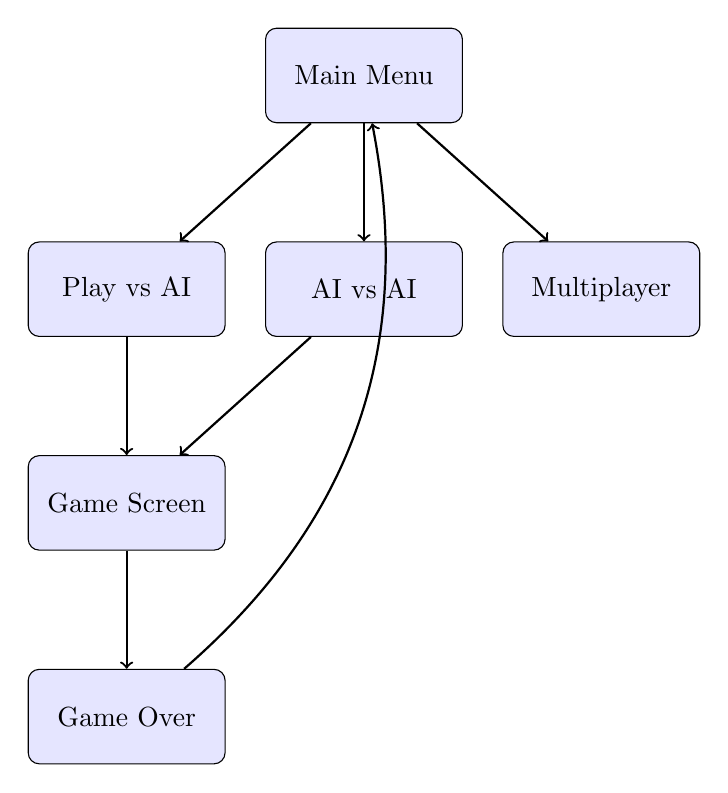
\begin{tikzpicture}[
    node distance=2cm,
    screen/.style={rectangle, draw, rounded corners, minimum width=2.5cm, minimum height=1.2cm, fill=blue!10},
    arrow/.style={->, thick}
]
    \node[screen] (menu) {Main Menu};
    \node[screen, below left=1.5cm and 0.5cm of menu] (play) {Play vs AI};
    \node[screen, below=1.5cm of menu] (aivsai) {AI vs AI};
    \node[screen, below right=1.5cm and 0.5cm of menu] (multi) {Multiplayer};
    \node[screen, below=1.5cm of play] (game) {Game Screen};
    \node[screen, below=1.5cm of game] (end) {Game Over};
   
    \draw[arrow] (menu) -- (play);
    \draw[arrow] (menu) -- (aivsai);
    \draw[arrow] (menu) -- (multi);
    \draw[arrow] (play) -- (game);
    \draw[arrow] (aivsai) -- (game);
    \draw[arrow] (game) -- (end);
    \draw[arrow, bend right=30] (end) to (menu);
\end{tikzpicture}
\caption{GUI Screen Flow Diagram}
\label{fig:gui_flow}
\end{figure}
\subsubsection{Main Menu Features}
\begin{table}[H]
\centering
\begin{tabular}{lp{8cm}}
\toprule
\textbf{Component} & \textbf{Description} \\
\midrule
Model Selector & Dropdown menu to choose AI opponent from discovered models \\
Play vs AI & Human player vs selected AI model \\
AI vs AI & Spectator mode watching two AIs compete \\
Multiplayer (3-4) & Launch multiplayer GUI with 3-4 players \\
Battle Arena & Open model comparison interface \\
Quit & Exit application \\
\bottomrule
\end{tabular}
\caption{Main Menu Components}
\label{tab:main_menu}
\end{table}

\subsubsection{Game Screen Layout}
\begin{figure}[H]
\centering
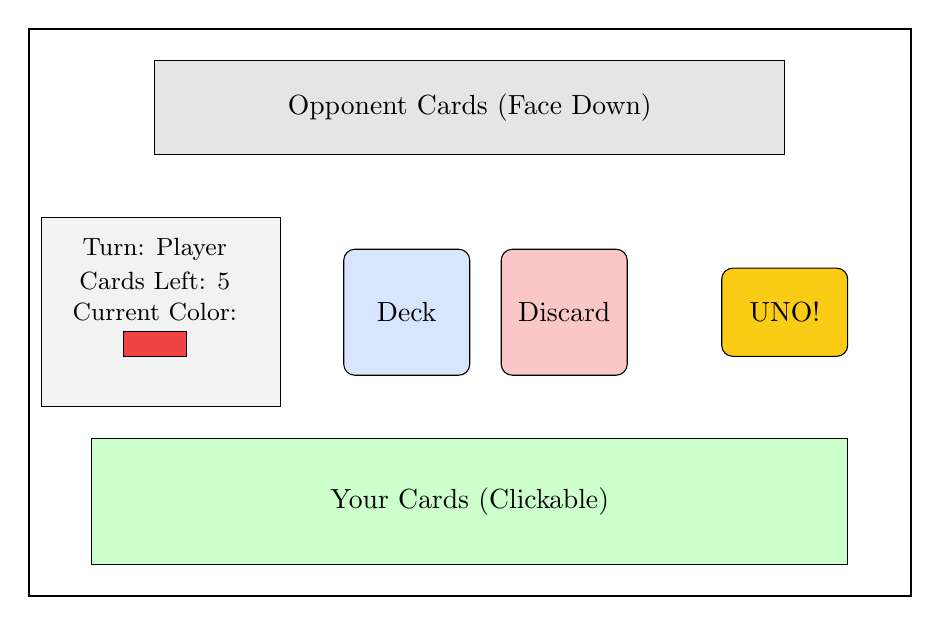
\begin{tikzpicture}[scale=0.8]
    % Screen outline
    \draw[thick] (0,0) rectangle (14,9);
   
    % Opponent area
    \draw[fill=gray!20] (2,7) rectangle (12,8.5);
    \node at (7,7.75) {Opponent Cards (Face Down)};
    
   
    % Center area
    \draw[fill=unoBlue!20, rounded corners] (5,3.5) rectangle (7,5.5);
    \node at (6,4.5) {Deck};
   
    \draw[fill=unoRed!30, rounded corners] (7.5,3.5) rectangle (9.5,5.5);
    \node at (8.5,4.5) {Discard};
   
    % Player area
    \draw[fill=green!20] (1,0.5) rectangle (13,2.5);
    \node at (7,1.5) {Your Cards (Clickable)};
   
    % UNO button
    \draw[fill=unoYellow, rounded corners] (11,3.8) rectangle (13,5.2);
    \node at (12,4.5) {UNO!};
   
    % Info panel
    \draw[fill=gray!10] (0.2,3) rectangle (4,6);
    \node[font=\small] at (2,5.5) {Turn: Player};
    \node[font=\small] at (2,5) {Cards Left: 5};
    \node[font=\small] at (2,4.5) {Current Color:};
    \draw[fill=unoRed] (1.5,3.8) rectangle (2.5,4.2);
   
\end{tikzpicture}
\caption{Game Screen Layout}
\label{fig:game_layout}
\end{figure}

\subsection{Model Battle Arena (model\_battle\_gui.py)}
\subsubsection{Purpose}
The Battle Arena allows systematic comparison of different AI models through automated batch evaluation.
\subsubsection{Features}
\begin{itemize}
    \item \textbf{2-4 Player Battles}: Configure matches with 2, 3, or 4 players
    \item \textbf{Multiple Model Selection}: Independent model selector for each player
    \item \textbf{Batch Evaluation}: Run 10 to 1000 games automatically
    \item \textbf{Real-time Statistics}: Win counts, percentages, average turns
    \item \textbf{Progress Tracking}: Visual progress bar during batch runs
    \item \textbf{CSV Export}: Save results for external analysis
\end{itemize}

\subsubsection{Battle Arena Layout}
\begin{figure}[H]
\centering
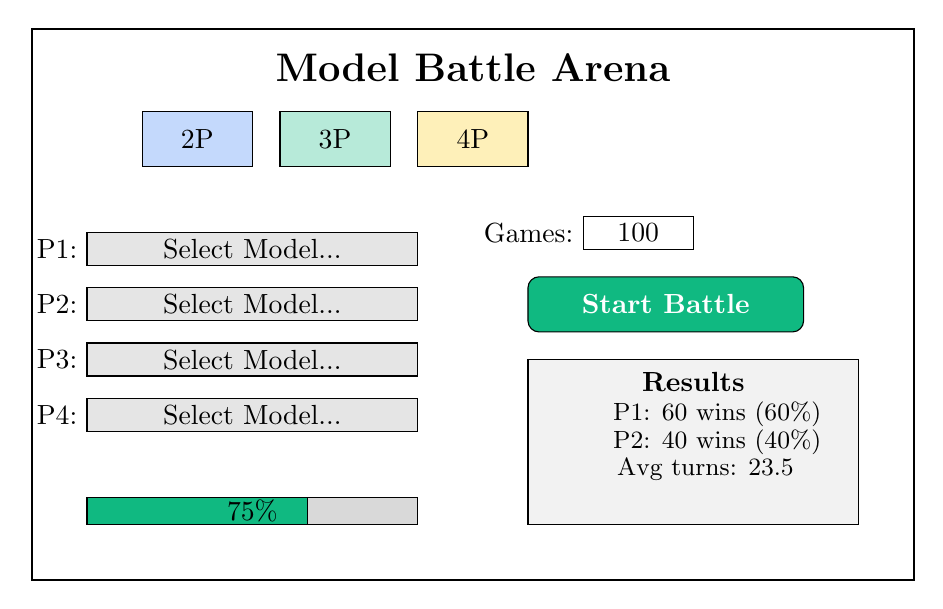
\begin{tikzpicture}[scale=0.7]
    % Screen outline
    \draw[thick] (0,0) rectangle (16,10);
   
    % Title
    \node[font=\Large\bfseries] at (8,9.3) {Model Battle Arena};
   
    % Player count buttons
    \draw[fill=unoBlue!30] (2,7.5) rectangle (4,8.5);
    \node at (3,8) {2P};
    \draw[fill=unoGreen!30] (4.5,7.5) rectangle (6.5,8.5);
    \node at (5.5,8) {3P};
    \draw[fill=unoYellow!30] (7,7.5) rectangle (9,8.5);
    \node at (8,8) {4P};
   
    % Model selectors
    \foreach \i/\y in {1/6, 2/5, 3/4, 4/3} {
        \draw[fill=gray!20] (1,\y-0.3) rectangle (7,\y+0.3);
        \node[left] at (1,\y) {P\i:};
        \node at (4,\y) {Select Model...};
    }
   
    % Game count input
    \draw[fill=white] (10,6) rectangle (12,6.6);
    \node[left] at (10,6.3) {Games:};
    \node at (11,6.3) {100};
   
    % Start button
    \draw[fill=unoGreen, rounded corners] (9,4.5) rectangle (14,5.5);
    \node[white, font=\bfseries] at (11.5,5) {Start Battle};
   
    % Results panel
    \draw[fill=gray!10] (9,1) rectangle (15,4);
    \node[font=\bfseries] at (12,3.6) {Results};
    \node[font=\small, left] at (14.5,3) {P1: 60 wins (60\%)};
    \node[font=\small, left] at (14.5,2.5) {P2: 40 wins (40\%)};
    \node[font=\small, left] at (14,2) {Avg turns: 23.5};
   
    % Progress bar
    \draw[fill=gray!30] (1,1) rectangle (7,1.5);
    \draw[fill=unoGreen] (1,1) rectangle (5,1.5);
    \node at (4,1.25) {75\%};
   
\end{tikzpicture}
\caption{Battle Arena Interface Layout}
\label{fig:battle_layout}
\end{figure}

\subsection{Multiplayer GUI (multiplayer\_gui.py)}
\subsubsection{Purpose}
Extends the game to support 3-4 players with proper turn direction handling.
\subsubsection{Key Differences from 2-Player}
\begin{table}[H]
\centering
\begin{tabular}{lll}
\toprule
\textbf{Feature} & \textbf{2-Player} & \textbf{3-4 Player} \\
\midrule
Reverse Card & Acts as Skip & Changes turn direction \\
Turn Direction & N/A & Clockwise/Counter-clockwise \\
Skip Card & Opponent skipped & Next player skipped \\
Display Layout & Top/Bottom & Circular arrangement \\
Observation & 17 dimensions & 25 dimensions \\
\bottomrule
\end{tabular}
\caption{2-Player vs Multiplayer Differences}
\label{tab:multi_diff}
\end{table}

\subsubsection{Turn Direction Visualization}
\begin{figure}[H]
\centering
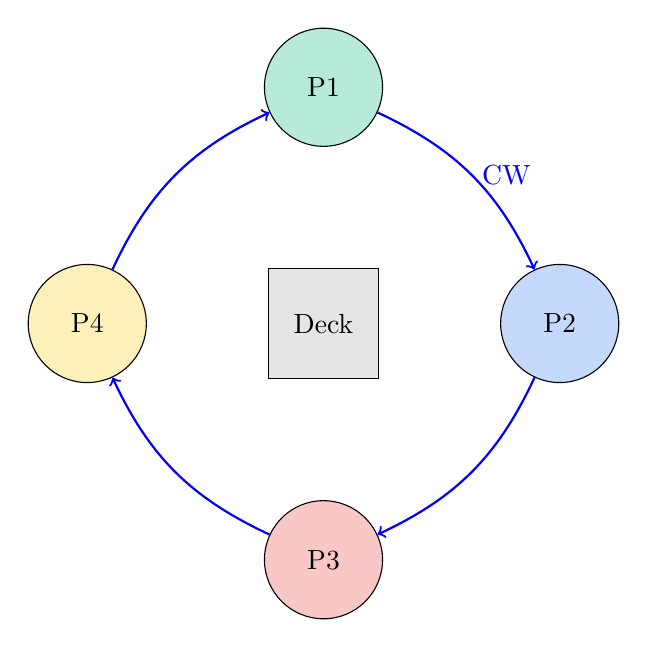
\begin{tikzpicture}
    % Players
    \node[circle, draw, fill=unoGreen!30, minimum size=1.5cm] (p1) at (0,3) {P1};
    \node[circle, draw, fill=unoBlue!30, minimum size=1.5cm] (p2) at (3,0) {P2};
    \node[circle, draw, fill=unoRed!30, minimum size=1.5cm] (p3) at (0,-3) {P3};
    \node[circle, draw, fill=unoYellow!30, minimum size=1.5cm] (p4) at (-3,0) {P4};
   
    % Clockwise arrows
    \draw[->, thick, blue] (p1) to[bend left=20] node[right] {CW} (p2);
    \draw[->, thick, blue] (p2) to[bend left=20] (p3);
    \draw[->, thick, blue] (p3) to[bend left=20] (p4);
    \draw[->, thick, blue] (p4) to[bend left=20] (p1);
   
    % Center
    \draw[fill=gray!20] (-0.7,-0.7) rectangle (0.7,0.7);
    \node at (0,0) {Deck};
\end{tikzpicture}
\caption{4-Player Circular Layout with Turn Direction}
\label{fig:multi_layout}
\end{figure}
\subsection{Design Philosophy: Glassmorphism}


\textbf{Design Elements:}
\begin{itemize}
    \item Semi-transparent backgrounds with blur effect simulation
    \item Subtle gradients and shadows
    \item Rounded corners on all interactive elements
    \item Color-coded UNO cards matching official colors
    \item Smooth hover and click animations
    \item Consistent 60 FPS rendering
\end{itemize}
\newpage
% ============================================================================
\section{Advanced Features}
\label{sec:advanced}
% ============================================================================
\subsection{Self-Play Training System}
\subsubsection{Architecture}
Self-play training improves performance by creating an adaptive curriculum of opponents.
\begin{figure}[H]
\centering
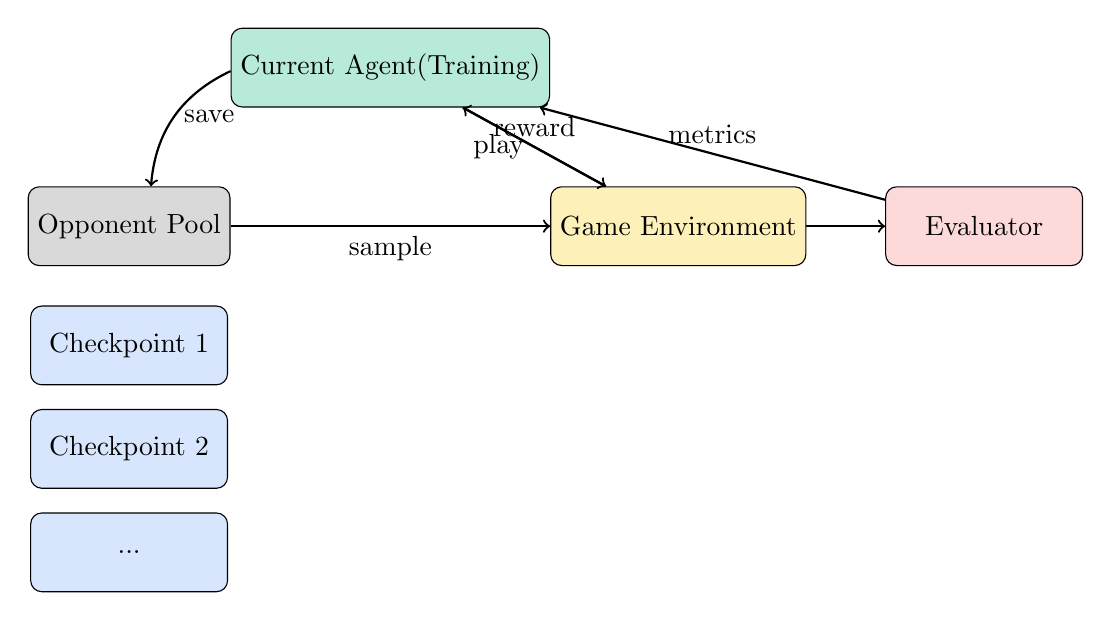
\begin{tikzpicture}[
    node distance=1.5cm,
    box/.style={rectangle, draw, rounded corners, minimum width=2.5cm, minimum height=1cm, fill=blue!10},
    arrow/.style={->, thick}
]
    \node[box, fill=unoGreen!30] (current) {Current Agent\\(Training)};
    \node[box, fill=gray!30, below left=1cm and 0cm of current] (pool) {Opponent Pool};
    \node[box, fill=unoBlue!20, below=0.5cm of pool] (chk1) {Checkpoint 1};
    \node[box, fill=unoBlue!20, below=0.3cm of chk1] (chk2) {Checkpoint 2};
    \node[box, fill=unoBlue!20, below=0.3cm of chk2] {...};
    \node[box, fill=unoYellow!30, below right=1cm and 0cm of current] (env) {Game Environment};
    \node[box, fill=unoRed!20, right=1cm of env] (eval) {Evaluator};
   
    \draw[arrow] (current) -- node[left] {play} (env);
    \draw[arrow] (pool) -- node[below] {sample} (env);
    \draw[arrow] (env) -- node[above] {reward} (current);
    \draw[arrow] (current) to[bend right=30] node[right] {save} (pool);
    \draw[arrow] (eval) -- node[above] {metrics} (current);
    \draw[arrow] (env) -- (eval);
\end{tikzpicture}
\caption{Self-Play Training Architecture}
\label{fig:selfplay_arch}
\end{figure}
\subsubsection{Training Phases}
\begin{enumerate}
    \item \textbf{Phase 1: Foundation (0-100K steps)}
    \begin{itemize}
        \item Train against random opponents
        \item Learn basic valid move selection
        \item Establish baseline policy
    \end{itemize}
   
    \item \textbf{Phase 2: Self-Play Introduction (100K-500K steps)}
    \begin{itemize}
        \item Mix of random (30\%) and self (70\%) opponents
        \item Start saving checkpoints to opponent pool
        \item Learn intermediate strategies
    \end{itemize}
   
    \item \textbf{Phase 3: Pure Self-Play (500K+ steps)}
    \begin{itemize}
        \item Primarily self-play with population sampling
        \item Curriculum of increasingly difficult opponents
        \item Target 70\%+ win rate against random
    \end{itemize}
\end{enumerate}

\newpage
\subsection{Multiplayer Environment}
\subsubsection{Extended State Representation}
For 3-4 players, the observation space expands to 25 dimensions:
\begin{table}[H]
\centering
\begin{tabular}{clc}
\toprule
\textbf{Index} & \textbf{Feature} & \textbf{Encoding} \\
\midrule
0-3 & Open card color & One-hot \\
4-7 & Number cards per color & Normalized count \\
8-10 & Special cards (Skip/Rev/+2) & Normalized count \\
11-12 & Wild cards (Wild/+4) & Normalized count \\
13-16 & Playable colors & Binary \\
17-20 & Opponent 1 hand size & Bucketed one-hot \\
21-24 & Opponent 2 hand size & Bucketed one-hot \\
\bottomrule
\end{tabular}
\caption{25-Dimensional Multiplayer Observation Space}
\label{tab:multi_obs}
\end{table}
\textbf{Hand Size Bucketing:}
\begin{itemize}
    \item Bucket 0: 0 cards (won)
    \item Bucket 1: 1-3 cards (UNO danger)
    \item Bucket 2: 4-6 cards (normal)
    \item Bucket 3: 7+ cards (high count)
\end{itemize}
\newpage
\section{Conclusion}
\label{sec:conclusion}
% ============================================================================
\subsection{Summary of Achievements}
This project successfully developed a comprehensive reinforcement learning system for the UNO card game:
\begin{itemize}
    \item \textbf{Complete Game Engine}: Full UNO implementation with all card types and rules
    \item \textbf{Multiple RL Algorithms}: Q-Learning, DQN, A2C, PPO, and RecurrentPPO
    \item \textbf{High Performance}: 60\% win rate with RecurrentPPO (2.4x random baseline)
    \item \textbf{Self-Play Training}: Framework targeting 70\%+ win rates
    \item \textbf{Modern GUIs}: Three Pygame interfaces with glassmorphism design
    \item \textbf{Multiplayer Support}: 2-4 player environments and gameplay
    \item \textbf{Comprehensive Documentation}: Full API docs and user guides
\end{itemize}
\subsection{Key Technical Contributions}
\subsubsection{Algorithm Insights}
\begin{enumerate}
    \item \textbf{Recurrent architectures are essential} for partially observable games
    \item \textbf{LSTM hidden size of 256} provides optimal performance/efficiency
    \item \textbf{Entropy coefficient of 0.01} prevents premature convergence
    \item \textbf{Self-play with curriculum} accelerates learning significantly
\end{enumerate}
\subsubsection{Engineering Contributions}
\begin{enumerate}
    \item Gymnasium-compatible UNO environment with 17/25-dim observations
    \item Modular architecture supporting easy algorithm swapping
    \item Efficient batch evaluation system for model comparison
    \item Production-ready GUI with model hot-swapping
\end{enumerate}
\subsection{Limitations}
\begin{itemize}
    \item \textbf{Partial Observability}: Even LSTM cannot perfectly infer hidden information
    \item \textbf{Opponent Diversity}: Models trained against limited opponent types
    \item \textbf{Computational Cost}: RecurrentPPO requires significant training time
    \item \textbf{Rule Variations}: Only standard UNO rules implemented
\end{itemize}
\subsection{Future Work}
\subsubsection{Short-Term Goals}
\begin{enumerate}
    \item Achieve 70\%+ win rate through extended self-play training
    \item Implement opponent modeling for hand prediction
    \item Add tournament mode for multi-model competition
    \item Create web-based interface for broader accessibility
\end{enumerate}
\subsubsection{Long-Term Goals}
\begin{enumerate}
    \item \textbf{Transformer Architectures}: Replace LSTM with attention mechanisms
    \item \textbf{Multi-Agent RL}: Train multiple agents simultaneously
    \item \textbf{Transfer Learning}: Apply learned strategies to other card games
    \item \textbf{Online Multiplayer}: Real-time human vs AI over network
    \item \textbf{Explainable AI}: Visualize agent decision-making process
\end{enumerate}
\subsection{Lessons Learned}
\begin{importantbox}
\textbf{Key Takeaway}: For games with partial observability and sequential decision-making, recurrent neural networks provide significant advantages over feedforward architectures. The LSTM's ability to maintain memory of past observations is crucial for inferring hidden game state.
\end{importantbox}
\newpage
% ============================================================================
\section*{Appendix A: Installation Guide}
\addcontentsline{toc}{section}{Appendix A: Installation Guide}
% ============================================================================
\subsection*{System Requirements}
\begin{itemize}
    \item Python 3.10 or higher
    \item 8GB RAM minimum (16GB recommended for training)
    \item NVIDIA GPU with CUDA support (optional, for faster training)
    \item Windows 10/11, Linux, or macOS
\end{itemize}
\subsection*{Installation Steps}
\lstset{language=bash}
\begin{lstlisting}
# Clone repository
git clone https://github.com/user/uno-card-game-rl.git
cd uno-card-game-rl
# Create virtual environment
python -m venv .venv
# Activate (Windows)
.venv\Scripts\activate
# Activate (Linux/macOS)
source .venv/bin/activate
# Install dependencies
pip install -r requirements.txt
# Verify installation
python -c "from sb3_contrib import RecurrentPPO; print('OK')"
# Run the game
python uno_gui.py
\end{lstlisting}
\subsection*{Dependencies}
\begin{lstlisting}
# requirements.txt
torch>=2.0.0
stable-baselines3>=2.0.0
sb3-contrib>=2.0.0
gymnasium>=0.29.0
pygame>=2.5.0
numpy>=1.24.0
pandas>=2.0.0
matplotlib>=3.7.0
tensorboard>=2.14.0
\end{lstlisting}
\newpage
% ============================================================================
\section*{Appendix B: Quick Reference}
\addcontentsline{toc}{section}{Appendix B: Quick Reference}
% ============================================================================
\subsection*{Command Reference}
\begin{table}[H]
\centering
\begin{tabular}{lp{8cm}}
\toprule
\textbf{Command} & \textbf{Description} \\
\midrule
\texttt{python uno\_gui.py} & Launch main game GUI \\
\texttt{python model\_battle\_gui.py} & Launch battle arena \\
\texttt{python multiplayer\_gui.py} & Launch multiplayer mode \\
\texttt{python train\_rl.py --algorithm ppo} & Train PPO model \\
\texttt{python train\_recurrent\_ppo.py} & Train RecurrentPPO \\
\texttt{python training/train\_selfplay.py} & Self-play training \\
\texttt{python compare\_models.py} & Evaluate models \\
\texttt{tensorboard --logdir logs/} & View training logs \\
\bottomrule
\end{tabular}
\caption{Command Reference}
\label{tab:commands}
\end{table}
\subsection*{Model Files}
\begin{table}[H]
\centering
\begin{tabular}{llc}
\toprule
\textbf{File} & \textbf{Algorithm} & \textbf{Win Rate} \\
\midrule
\texttt{selfplay\_champion.zip} & RecurrentPPO & 70\%+ \\
\texttt{best\_recurrent\_ppo.zip} & RecurrentPPO & 60\% \\
\texttt{optimal\_recurrent\_ppo.zip} & RecurrentPPO & 59\% \\
\texttt{sb3\_recurrent\_ppo.zip} & RecurrentPPO & 57\% \\
\texttt{best\_ppo.zip} & PPO & 53\% \\
\texttt{dqn\_uno.zip} & DQN & 48\% \\
\texttt{a2c\_uno.zip} & A2C & 45\% \\
\bottomrule
\end{tabular}
\caption{Model Files}
\label{tab:model_files}
\end{table}
\newpage
% ============================================================================
\section*{Appendix C: Hyperparameter Reference}
\addcontentsline{toc}{section}{Appendix C: Hyperparameter Reference}
% ============================================================================
\begin{table}[H]
\centering
\begin{tabular}{lccc}
\toprule
\textbf{Parameter} & \textbf{PPO} & \textbf{RecurrentPPO} & \textbf{Effect} \\
\midrule
learning\_rate & 3e-4 & 2.5e-4 & Training speed/stability \\
n\_steps & 2048 & 128 & Rollout length \\
batch\_size & 64 & 256 & Mini-batch size \\
n\_epochs & 10 & 4 & Updates per rollout \\
gamma & 0.99 & 0.99 & Discount factor \\
gae\_lambda & 0.95 & 0.95 & GAE parameter \\
clip\_range & 0.2 & 0.2 & PPO clipping \\
ent\_coef & 0.01 & 0.01 & Exploration bonus \\
vf\_coef & 0.5 & 0.5 & Value loss weight \\
lstm\_hidden & - & 256 & LSTM units \\
\bottomrule
\end{tabular}
\caption{Recommended Hyperparameters}
\label{tab:hyper_ref}
\end{table}
\end{document}